\documentclass[book]{deliverablereport}

\usepackage[style=alphabetic,backend=biber]{biblatex}
\addbibresource{../../lib/kbibs/kwarcpubs.bib}
\addbibresource{../../lib/kbibs/extpubs.bib}
\addbibresource{../../lib/kbibs/kwarccrossrefs.bib}
\addbibresource{../../lib/kbibs/extcrossrefs.bib}
\addbibresource{../../lib/deliverables.bib}
\addbibresource{local.bib}
% temporary fix due to http://tex.stackexchange.com/questions/311426/bibliography-error-use-of-blxbblverbaddi-doesnt-match-its-definition-ve
\makeatletter\def\blx@maxline{77}\makeatother
\usepackage{local}
\usepackage[hide]{ed}

\title{OEIS Case Study (Coverage and Automated Import)}
\def\shorttitle{Report on \pn D6.2 and D6.3}

\deliverable{dksbases}{conv}
\deliverydate{1/09/2017}
\duedate{1/09/2018}

\author{Enxhell Luzhnica}
\author{Michael Kohlhase}


\begin{document}
\begin{abstract}\strut\\
  {\color{red} This is an interrim report for the OEIS part of this deliverable (reference
    it as ODK Report D6.4.2) which has been completed ahead of time. This report is
    largely based on the thesis \cite{Luzhnica:bsc16}.}

  \begin{sffamily}
  The On-line Encyclopedia of Integer Sequences (\oeis) is the largest database of its
  kind and an important resource for mathematicians. The database is well-structured and
  rich in mathematical content but is informal in nature, so knowledge management services
  are not directly applicable.  In this report we provide a partial parser for the \oeis
  that leverages the fact that, in practice, the syntax used in its formulas is fairly
  regular. Then, we import the result into \omdoc to make the \oeis accessible to
  \omdoc-based knowledge management applications. We exemplify this with a formula search
  application based on the \mws system and a program that finds relations between the
  \oeis sequences.  In addition, we design a new formula language for the \oeis and build
  a parser for it.
  \end{sffamily}
\end{abstract}
\maketitle
%\newpage\strut\githubissuedescription

\newpage
\tableofcontents
\newpage
\chapter{Conversion of the LMFDB}
This part will be added later. 

\chapter{Conversion of the OEIS}
\section{Introduction}\label{sec:intro}

\begin{newpart}{MK: adapted from Tom's Thesis}
There is a large and vibrant ecosystem of open-source mathematical software systems.
These systems can range from calculators, which are only capable of performing simple
computations, via mathematical databases (curating collections of a mathematical objects)
to powerful modeling tools and computer algebra systems (CAS). 

Most of these systems are very specific -- they focus on one or very few aspects of
mathematics.  For example, the ``Online Encyclopedia of Integer Sequences''
(OEIS~\cite{Sloane:oeis12,oeis}) focuses on sequences over $\mathbb{Z}$ an their
properties and the ``L-Functions and Modular Forms Database''
(LMFDB)~\cite{Cremona:LMFDB16,lmfdb:on} objects in number theory pertaining to Langland's
program.  GAP~\cite{GAP:on} excels at discrete algebra, whereas
SageMath~\cite{SageMath:on} focuses on Algebra and Geometry in general, and
Singular~\cite{singular:on} on polynomial computations, with special emphasis on
commutative and non-commutative algebra, algebraic geometry, and singularity theory.

For a mathematician however (a user; let us call her Jane) the systems themselves are not relevant, instead she only cares about being able to solve problems. 
Typically, it is not possible to solve a mathematical problem using only a single program. 
Thus Jane needs to work with multiple systems and combine the results to reach a solution. 
Currently there is very little help with this practice, so Jane has to isolate sub-problems the respective systems are amenable to, formulate them into the respective input language, collect results, and reformulate them for the next system a tedious and error-prone process at best, a significant impediment to scientific progress in its overall effect. 
Solutions for some situations certainly exist, which can help get Jane unstuck, but these are ad-hoc and for specific, often-used system combinations only. 
Each of these requires a lot of maintenance and does not scale to a larger set of specialist systems. 

The OpenDreamKit project, which aims at a mathematical VRE toolkit, proposes the Math-in-the-Middle (MitM~\cite{DehKohKon:iop16}) Paradigm, an interoperability framework based on a flexiformal
representation of mathematical knowledge and aligns this with system-generated interface
theories. 

In this paper we instantiate the MitM paradigm with a concrete domain development and
evaluate it on a distributed computing GAP, SageMath and Singular.\ednote{ we generally we
  want to show that the promises in the CICM paper become reality.}

We will use the following example as a running example: Jane wants to act on singular
polynomials with GAP permutation groups\ednote{MK@(MP|VA): }

 \ednote{MK: continue with the structure} 
\end{newpart}

%%% Local Variables:
%%% mode: latex
%%% TeX-master: "paper"
%%% End:

\section{Preliminaries} \label{sec:Preliminaries}

\subsection{The \oeis document format}\label{sec:doc-form}

The \emph{internal format} \cite{oeis-help} is line-based in the sense that
each line starts with a marker that represents the kind of content found 
in that line. We briefly introduce the relevant kinds below but refer to 
\cite{oeis-help} for details.

\begin{wrapfigure}{r}{9.5cm}
\vspace{-1.0cm}
\begin{center}
\begin{tabular}{|lll|}
\hline
\req{\textit{Ident.}} & \bbc & $\mathtt{\%I \;} \mathit{ID}\; \opt{M_n} \; \opt{N_n} $ \\
$\mathit{ID}$ & \bbc & Identification number in \cite{oeis} \\
$M_n$ & \bbc & Identification number in \cite{encyc-is} \\
$N_n$ & \bbc & Identification number in \cite{handbook-is} \\
\req{\textit{Values}} & \bbc & $\mathtt{\%S \; } \mathit{ID}\; \mathrm{nr}^\rep \; \opt{\mathtt{\%T \; 
ID}\; \mathrm{nr}^\rep \; \opt{\mathtt{\%U \; } \mathit{ID}\; \mathrm{nr}^\rep}} $ \\

\req{\textit{Name}} & \bbc & $\mathtt{\%N \; } \mathit{ID} \; \mathrm{text}$ \\
\textit{References} & \bbc & $\mathtt{\%D \; } \mathit{ID} \; \mathrm{text}$  \\
\textit{Formula} & \bbc & $\mathtt{\%F \; } \mathit{ID} \; \mathrm{formula}$  \\
\req{\textit{Author}} & \bbc & $\mathtt{\%A \; } \mathit{ID} \; \mathrm{text}$  \\
\textit{Examples} & \bbc & $\mathtt{\%E \; } \mathit{ID} \; \mathrm{text}$ \\
\hline

\end{tabular}
\caption{Grammar of \oeis Internal Format}\label{fig:int-form}
\end{center}
\end{wrapfigure}

\begin{compactenum}
 \item The \emph{identification} line gives the unique ID of the sequence declared in that document. 
 \item The \emph{start values} lines give the beginning of the sequence. It is used for searching as 
well as lexicographic ordering of the sequences.
 \item The \emph{name} line gives the name, a brief description or the definition of the sequence.
 \item The \emph{references} lines contain references to papers which in turn refer to or are concerned with the 
 sequence described in the current document.
 \item The \emph{formula} lines give formulas that define or hold for the sequence described in the current document. 
 The formulas are in plain text ASCII syntax that is similar to {\LaTeX} math markup and can contain text as 
 part of the formula or as comments. Among others, here we find the representing functions and the generating
 functions (starting with \texttt{G.f.}) of the sequence in hand.
 \item The \emph{author} line gives the document author typically containing the name and e-mail address.
 \item The \emph{examples} lines give examples and additional information about the initial terms of the sequences
\end{compactenum}

The actual document-level syntax of the internal format is presented below in Figure \ref{fig:int-form} where
we use \req{$\circ$} for required lines, $\opt{\circ}$ for optional parts, $\circ^\rep$ for repetitions and $\circ_1 
\alt \circ_2$ for alternatives. Moreover we use \textit{italic} for grammar productions, \texttt{typewriter font} for 
fixed syntax and normal font for informal descriptions.

[Fibonacci numbers]\label{ex:internal}
  The article for Fibonacci numbers \cite{oeis-fib} was one of the first entries in the
  \oeis and is one of the most comprehensive.  We will use it as a running example
  throughout the report, although we will heavily trim the document for simplicity by
  presenting here only a few sanitized lines. Listing
  \ref{lst:internal} shows the document with identification, values, name and reference
  lines, followed by three formula lines and the author line.

\begin{lstlisting}[caption=A000045,label=lst:internal,basicstyle=\scriptsize\sf]
%I A000045 M0692 N0256
%S A000045 0,1,1,2,3,5,8,13,21,34,55,89,144,233,377,610,987
%N A000045 Fibonacci numbers: F(n) = F(n-1) + F(n-2) with F(0) = 0 and F(1) = 1.
%D A000045 V. E. Hoggatt, Jr., Fibonacci and Lucas Numbers. Houghton, Boston, MA, 1969.
%F A000045 F(n) = ((1+sqrt(5))^n-(1-sqrt(5))^n)/(2^n*sqrt(5))
%F A000045 G.f.: Sum_{n>=0} x^n * Product_{k=1..n} (k + x)/(1 + k*x). - _Paul D. Hanna_, Oct 26 2013
%F A000045 This is a divisibility sequence; that is, if n divides m, then a(n) divides a(m)
%A A000045 _N. J. A. Sloane_, Apr 30 1991
\end{lstlisting}



\subsection{\omdmmt}

The \mmt language \cite{Rabe:MMTLanguageSystem09} is designed to be applicable to a large collection of declarative
formal base languages and all  \mmt notions are fully abstract in the choice of the base language. For clarification,
 typical base languages are logics, type theories, or programming languages. In \mmt, mathematical knowledge is
 defined in terms of four important
units: documents, modules, symbols and objects. The biggest unit of mathematical knowledge, the document, is
represented in  \mmt as a theory graph.
\textbf{Theory Graph} is one of the central notions of  \mmt which contains \emph{theories} or modules and
\emph{views} (morphisms between theories). To understand this better we will define some additional notions. \\
\textbf{Theories} are defined by a set of typed \textbf{symbols} (the signature) and a set of \textbf{axioms}
describing the properties of the symbols. \\
\textbf{Symbols} are either constant declarations (declaring constants, type axioms, lemmas, definitions) or a
structure declaration (which declares an import from another theory). In the latter case, all the symbols from the
imported theory become available. In the theory graph this is represented by an arrow from the imported theory to the importing one.
A \textbf{signature morphism} $\sigma$ from a source theory \emph{S} to a target theory \emph{T} translates or
interprets the symbols of \emph{S} in \emph{T}. \\
If we have entailment relations for the formulas of S and T, a signature morphism that translates all theorems of
\emph{S} to theorems of \emph{T} is called a \textbf{view}. So, in  \mmt a \textbf{view} from \emph{S} to \emph{T} is
 a list of assignments $c \mapsto \omega$ where $c$ is an \emph{S}-constant (axiom) and $\omega$ is a \emph{T}-term
 (proof). This list of assignments induces a homomorphic translation of S-terms to T-terms by replacing every $c$
 with the corresponding $\omega$.   \\
The object level provides the structure of the symbols inside a theory; objects are terms
produced by a grammar in which the basic units are constants, variables, applications and bindings. 

Let us consider the theories (Fig. \ref{img:graph}) of \textbf{group, monoid} and \textbf{unital set} of a monoid and
 one view \textbf{m} which shows that the unital set of a monoid is a group.

\begin{figure}[h!] 
\centerline{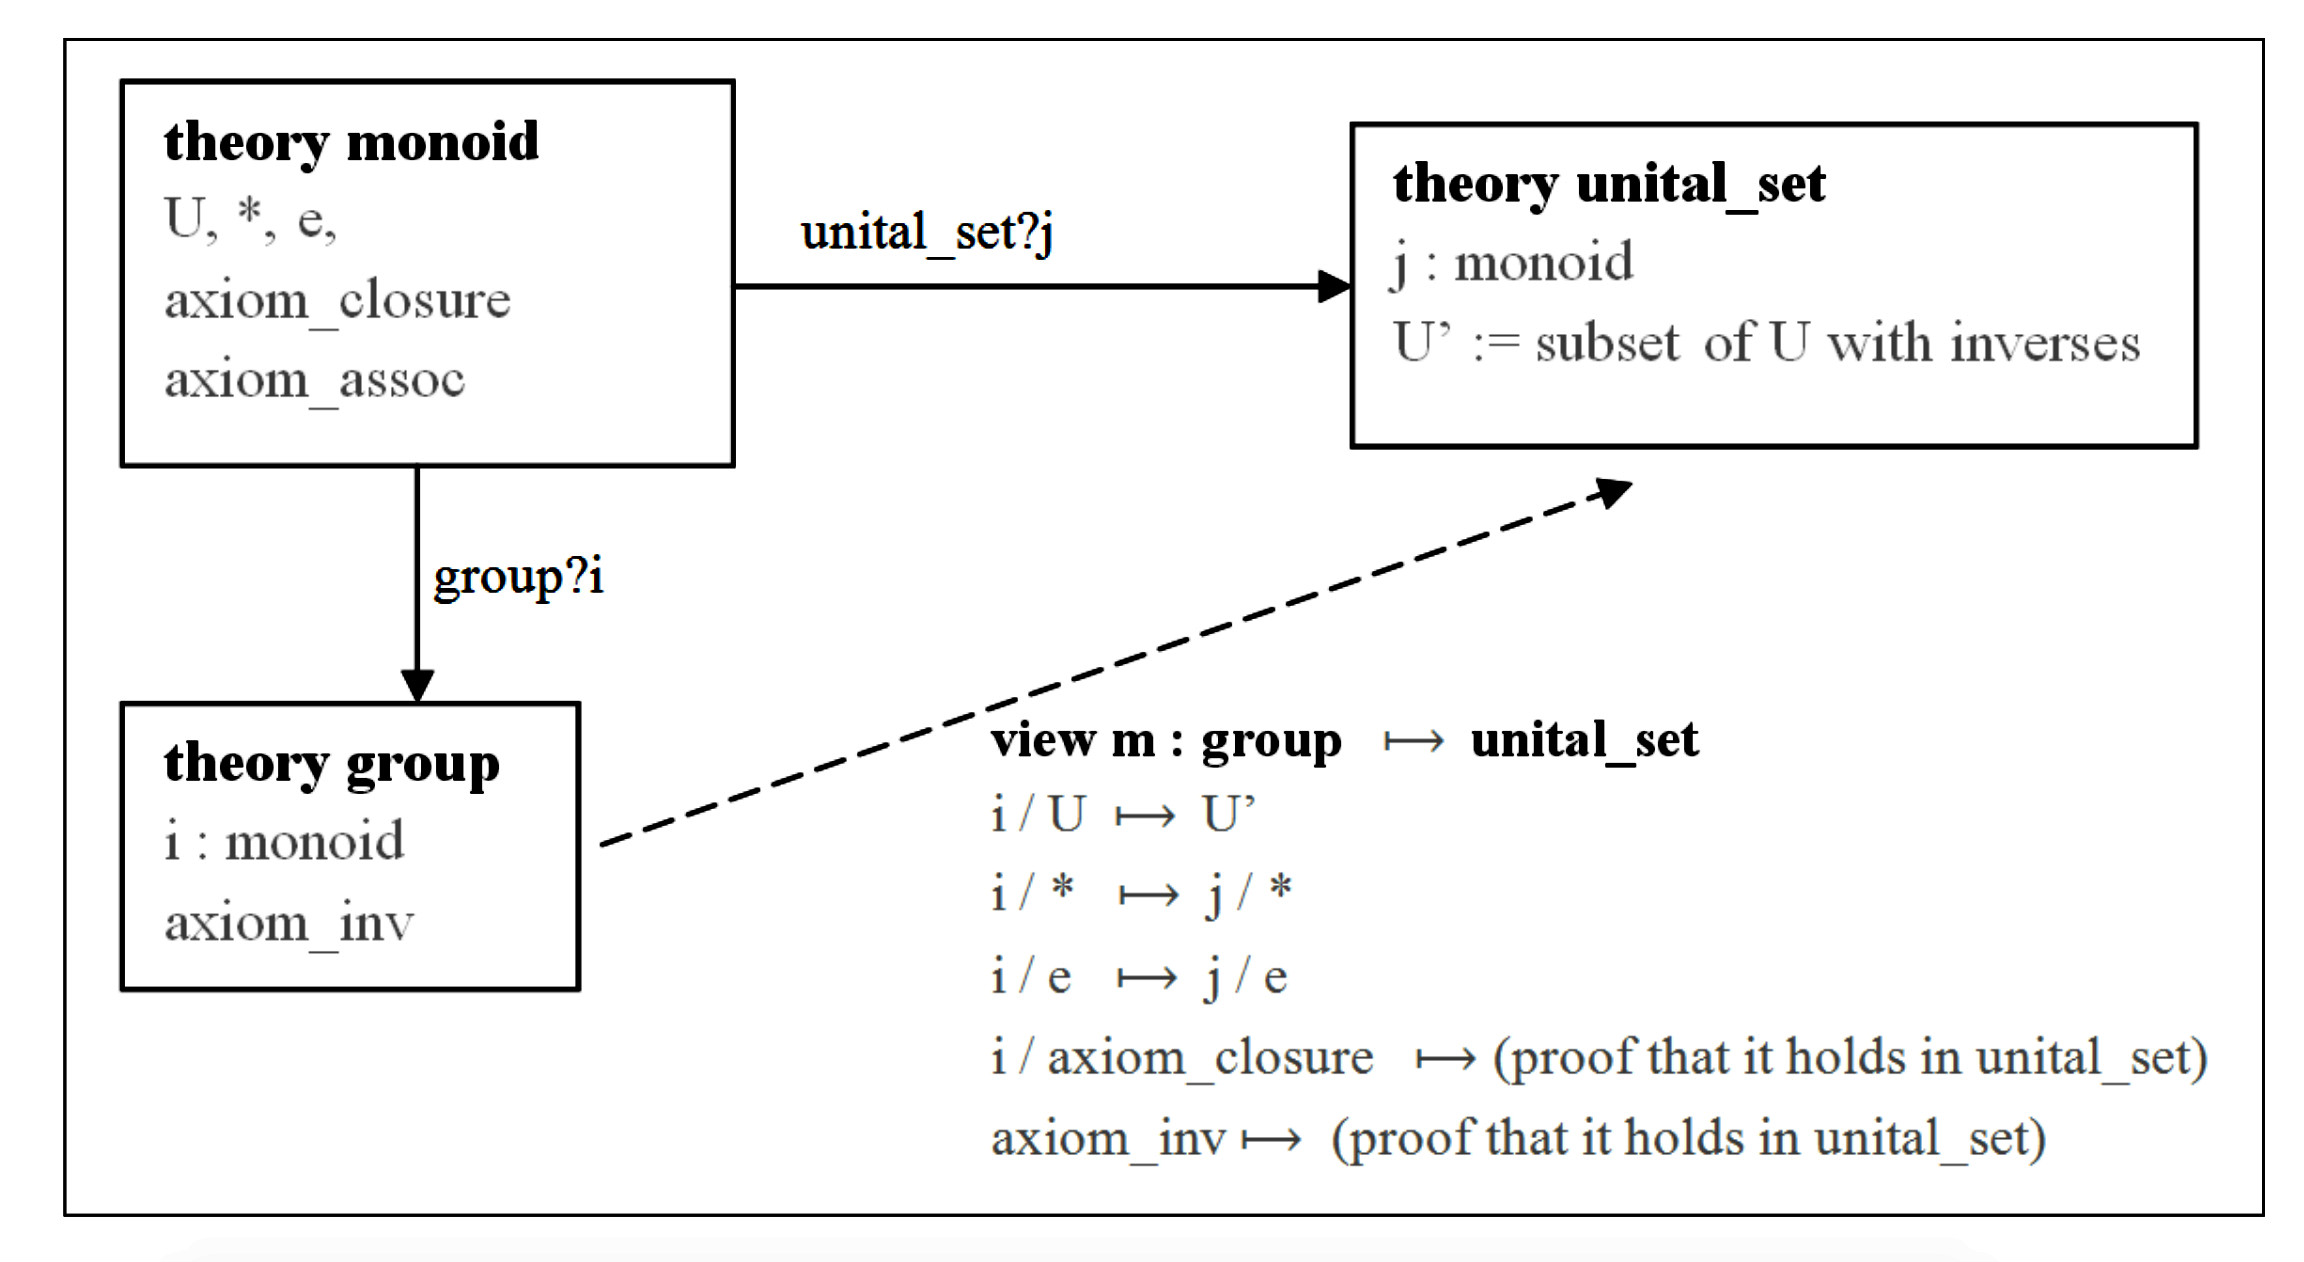
\includegraphics[scale=0.15]{theories1}}
\caption{An Example Theory Graph Comprising Three Theories \label{img:graph}}
\end{figure}

The imports (\textbf{unital\_set?j} and \textbf{group?i}) are marked by solid arrows. Each import carries all the
symbols from the source theory to the destination. In theory \textbf{monoid} the declared constants are
\textbf{U}-underlying set, $*$-monoid operation, \textbf{e}-unity element and \textbf{axiom\_closure, axiom\_assoc}.

Theory \textbf{group} imports from monoid via the structure \textbf{i} and formulates the axiom of invertibility.
Theory \textbf{unital\_set} imports from monoid via \textbf{j} and declares \textbf{U'}-the set of invertible
elements in \textbf{U}.
The view \textbf{m} is mapping all the symbols and proving the axioms still hold with the new mapping in
\textbf{unital\_set}.

\omdoc \cite{Kohlhase:OMDoc1.2} is a content markup format and data model for mathematical documents. It models
mathematical content using three levels.
\begin{compactdesc}
\item[Object Level:] uses {\openmath} and {\mathml} as established standards for
  the markup of \emph{formulae}.
\item[Statement Level:] supplies original markup for explicitly representing the
  various kinds of mathematical statements including \emph{symbol declarations} and \emph{definitions} (which
  introduce
a new symbol names), \emph{assertions} (which can represent theorems, lemmas or corollaries), and \emph{examples}.
\item[Theory Level:] offers original markup that allows for clustering sets
  of statements into \emph{theories} as well as specifying relations between them
  (inclusions, morphisms).
\end{compactdesc}
% \textbf{\omdoc} concentrates on the structural relations between these mathematical
% concepts. It deliberately avoids fixing language primitives for them and abstracts from
% specific mathematical foundations. This is a crucial design choice that makes {\omdoc} a
% universal representation format while remaining manageably simple.

The \mmt \cite{RabKoh:WSMSML13} language can be seen as a restricted version of \omdoc but
with a fully specified semantics. Additionally, for \mmt there is an \mmt system
\cite{Rabe:MAGMS13} which is a Scala-based \cite{scala:webpage} open source implementation
of the {\mmt} language. The key features of the \mmt system for this report are that it
provides an infrastructure for writing importers from any compatible format into \mmt as
well as exporters from \mmt, most notably into (\mathml-enriched) \html for both local and
web-based presentation.

For the sake of simplicity, we often do not differentiate between \mmt and \omdoc
languages in the following and refer to \cite{Kohlhase:OMDoc1.2} and, respectively,
\cite{RabKoh:WSMSML13} for details on each language. Throughout this report we will use
\omdmmt to refer to both \omdoc and \mmt.

\subsection{Theory of Generating Functions}
Generating functions are used to represent sequences efficiently by coding the terms of a sequence
as coefficients of powers of a variable $x$ in a formal power series.
Unlike an ordinary series, this formal series is allowed to diverge, meaning that the generating function is not
always a true function and the "variable" is actually an indeterminate.

Generating functions are used for solving combinatorial problems, recurrences and most importantly in our context,
analyzing various properties of sequences. There are different types of generating functions, including
\textbf{ordinary generating functions, exponential generating functions, Lambert series, Bell series}, and
\textbf{Dirichlet series}.

The \textbf{ordinary generating function} (or just \textbf{generating function}) of a sequence \\ $a_0, a_1, a_2
\ldots, a_{n-1}, a_n, \ldots$ is the infinite series:
\begin{equation}
GF(x) = a_0 + a_1x + a_2x^2 + \ldots + a_{n-1}x^{n-1} + a_nx^n + \ldots = \sum_{i=0}^{\infty} a_ix^i
\end{equation}

For example, the sequence $(1,1,1,1,1, \ldots)$ can be represented as:
\begin{equation}
1 + x + x^2 + \ldots = \frac{1}{1-x}
\end{equation}
We know that the equation above only holds for $|x|<1$ but we ignore the issues of convergence, as already mentioned.
 Thus, the ordinary generating function of this sequence can be written as $\frac{1}{1-x}$.

Due to this representation, generating functions have some interesting properties which we are going to discuss
shortly. Below are some properties of the ordinary generating functions.

Let $f(x) = \sum_{i=0}^{\infty} a_ix^i$, $g(x) = \sum_{i=0}^{\infty} b_ix^i$, $c \in \mathbb{R}$ and $k \in
\mathbb{Z}$, then
\begin{align}
f(x) + g(x) &= \sum_{i=0}^{\infty} (a_i + b_i) x^i \label{eq:add} \\
cf(x) &= \sum_{i=0}^{\infty} ca_ix^i \label{eq:scale} \\
x^kf(x) &= \sum_{i=0}^{\infty} a_ix^{i+k} \label{eq:shift} \\
\frac{d}{dx}f(x) &= \sum_{i=0}^{\infty} (i+1)a_{i+1}x^i \label{eq:diff} \\
\int f(x) dx &= \sum_{i=0}^{\infty} \frac{1}{i+1}a_ix^{i+1} \label{eq:int}
\end{align}
Equation \ref{eq:add} can be interpreted as adding two generating functions is the same as adding the sequences they
represent term by term. From equation \ref{eq:scale}, multiplying a generating function by some constant is the same
as multiplying each term of the sequence by that same constant. From equation \ref{eq:shift}, multiplying the
sequence by $x^k$ is the same as shifting the sequence to the left ($k<0$) or right ($k>0$). If shifted to the right,
 the new terms added in the beginning are $0$s. From equation \ref{eq:diff}, taking the derivative of a generating
 function is the same as multiplying each term by its index and shifting the sequence to the left by one. From
 equation \ref{eq:int}, taking the integral is the same as dividing each term by its index and shifting the sequence
 to the right by one.


%%% Local Variables:
%%% mode: latex
%%% TeX-master: "../report"
%%% End:

\section{Related Work and Comparisons} \label{sec:Related}

The content representation of mathematical expressions has been widely researched from
different perspectives. The main problem of processing natural language along a complex
mathematical symbolism has been mainly approached in two ways \cite{Ginev-11}. The first
approach tries to make a controlled natural language and make the language incrementally
more powerful while disallowing ambiguities. The ambiguity resolution here is usually
based on an explicit context and/or type inference. The top-down approach tries to model
the existing discourse of mathematics.  The parsing of mathematical expressions in done
mainly using context-free grammars aided with a type system or special purpose grammars
that are based on type systems. The work done using these approaches generally aims to
parse a large set of topics in the mathematical discourse. In our case we have a more
specific mathematical topic to parse and the discourse is only limited to mathematical
expressions. Our current approach is a top-down approach as we will see in Section
\ref{sec:form-parser}, although it is later amalgamated with techniques from the
controlled language approach by introducing a new formula language for \oeis.

On the other hand, the work in finding relations between sequences has been centered
around numerical based approaches, mainly due to the representation of the
\oeis. Generally, the high level approach is to apply different numerical transformations
on the available starting values of the integer sequences and then check for matches. This
match checking is usually done with exact matches on all starting values of a sequence or
only a subset of it, or even analyzing the sequence that comes out of some predefined
error function. Transformations are tuned for relations that the author is interested in,
keeping in mind the search costs. Two approaches of this nature have been compiled in
Appendix \ref{App:AppendixA}.

A disadvantage is that the found relations are only conjectures since the matching is done on a finite subsequence,
which usually is less than 30 terms. An extreme example of two sequences that match for a long time but are not
equal, is the following:

$$\floor*{\frac{2n}{log(2)}}  \qquad\text{and}\qquad \ceil*{\frac{2}{2^{1/n}-1}}$$

They agree for the first 777451915729367 terms \cite{oeis-paper2}!

In fact, a similar approach from Ralf Stephan \cite{Ralf} yielded 117 conjectures from
which 17 of them are still conjectures \cite{RalfUpdates}, which shows that these
conjectures are not always easy to prove or disprove.


%%% Local Variables:
%%% mode: latex
%%% TeX-master: "../report"
%%% End:

\section{Parsing the \oeis Formula Format}\label{sec:form-parser}
We built a partial parser for \oeis formulas by identifying
and analyzing well-behaved formulas to produce a workable grammar.
We leverage the fact that, although there is no standardized format for \oeis formulas, many of them use a
sufficiently
regular syntax.

\oeis is known for the human-readable mathematical terms, so a variety of syntactic rules are encountered when forming
these mathematical terms. We use the following classification for notations, inspired by \cite{ranta} and
further motivated by our analysis of the \oeis formulas:
\begin{compactenum}
\item \textbf{infix operators} are used to combine two terms to one complex term, e.g the \lstinline!+! symbol in
\lstinline!m+n!.
\item \textbf{suffix operators} are added after a term to form another term, e.g. the \lstinline|!| symbol in
\lstinline|n!|.
\item \textbf{prefix operators} (with or without bracketed application) are added in front of a term to form another
term,
e.g. \lstinline|sin| in \lstinline|sin(x)| or \lstinline|sin x|, respectively.
\item \textbf{infix relation symbols} are used to construct a formula out of two terms, e.g. the \lstinline|<| symbol
in \lstinline|x<2|.
\item \textbf{binding operators} that bind a context to a body to construct a term, e.g. the
\lstinline[mathescape]|$\forall$| symbol in
\lstinline[mathescape]|$\forall$x. x^2 > 0|
\end{compactenum}

The classification presented above guides our grammar and, in principle, covers virtually all important notations used
in \oeis formulas. However, in practice, we encountered several important challenges which we discuss individually
below.

\paragraph{Open Set of Primitives} Since the formulas are not standardized, not only is
the syntax flexible, but so is the set of primitive operators that are used. For instance,
the formulas in Listing \ref{lst:internal} (on lines $5$-$6$) use square root, power, as
well as the sum (\lstinline[mathescape]|$\Sigma$|) and product
(\lstinline[mathescape]|$\Pi$|) binders. The challenges arise because of the many
different notations used for such primitives. For instance, in line $6$ of Listing
\ref{lst:internal} the range for sum and product is given in two different ways. Similar
problems appear with limits and integrals as well as numerous atypical infix and suffix
operators.  In order to parse these correctly, we investigate the documents and the
grammar failures manually and incrementally extend the grammar.

\paragraph{Ambiguity}
As it is often the case with informal, presentation-oriented formulas, there can be
ambiguity in the parsing process when there exist several reasonable
interpretations. Since the \oeis syntax is not fixed, this is quite common, so we do
additional disambiguation during parsing to resolve most of the ambiguities. Here we
discuss a few of the many ambiguities that arise.

The multiplication sign is usually implicit so, instead of \lstinline!a*(x+y)!, we
encounter \lstinline!a(x+y)! which could represent either a function application or a
multiplication depending on whether \lstinline!a! is a function or an individual (constant
or variable).  There is no general way to solve this, so we rely on several
heuristics. First, we check if the symbol in question is used somewhere else in the same
formula with an unambiguous meaning.  Specifically, we default to function application
unless the same symbol is used as an individual somewhere else in the formula. This
already disambiguates most such cases in \oeis but we use several additional
heuristics. For instance, having \lstinline[mathescape]!name($arg$)! will result in
marking \lstinline!name! as function since it is unlikely to be a multiplication between
two individuals. Similarly, having \lstinline[mathescape]!name($arg_1$,...,$arg_n$)!
results in marking \lstinline!name! as a function.

The natural way of using the power operator also leads to ambiguities. For example,
\lstinline!T^2(y)! is used for $(T(y))^2$, however \lstinline!T^y(x^2+2)! is ambiguous.
We solve this using similar heuristics as for the implicit multiplication.

For unbracketed function application as in \lstinline!sin x!, we rely on the heuristic that this form of function
application is used only in well known functions. Therefore, we code these notations for well known
functions in the grammar itself. This form of function application can also mean multiplication, for instance
\lstinline!Pi x!.
One can already see that parsing and disambiguating the mathematical expressions in this context has a lot of aspects.
Additional cases of ambiguities are handled in similar ways and we omit the details for brevity.

\paragraph{Delineating formulas}
\oeis formula lines freely mix text and formulas so it is required to correctly distinguish between text and formula
parts within the lines in order to accurately parse each line. For instance, line $6$ in Listing
\ref{lst:internal} starts with the text \lstinline!G.f.:! (meaning ``Generating function:'') and continues with the
formula. The line then has the author and date, separated from the formula by a dash (\lstinline!-!) which
could also be interpreted as a minus and, therefore, a continuation of the formula.
In the extraction of the formulas we use the help of a dictionary. The text in the \oeis documents has words
that are not found in the dictionaries since it contains many technical terms so we first run a
pre-parsing procedure which enriches the dictionary. The final grammar tries to parse words until it fails and then
tries to parse formulas; this process repeats.

\subsection{Importing into \omdmmt}
For each \oeis document we create a corresponding \omdmmt document that contains a single theory. Then, \oeis lines
roughly correspond to \omdmmt declarations inside that theory. We use the \oeis sequence ID as the name of the \omdoc
theory. Then, the identification line produces an \omdoc symbol declaration representing the sequence (as a function
from integers to values). The start values and example lines are both represented as \omdmmt examples. Specifically,
the starting values are considered as examples of sequence elements. Formula lines are represented as \omdoc
assertions
(about the sequence symbol). Finally, name, reference and author lines are represented as metadata using the Dublin
Core standard.

[Fibonacci Numbers]\label{ex:omdoc}
 The corresponding \omdmmt document for the Fibonacci numbers article from Example \ref{ex:internal} is shown
 in Listing \ref{lst:omdoc}. We omit most formulas and some XML boilerplate for conciseness and simplicity.

 \begin{lstlisting}[mathescape,label=lst:omdoc]
  <omdoc xmlns:dc="http://purl.org/dc/elements/1.1/">
    <theory id="A000045">
    <metadata>
      <dc:creator>N. J. A. Sloane</dc:creator>
      <dc:title>Fibonacci numbers</dc:title>
    </metadata>
    <symbol name="seq"/>
    <assertion>
      <!-- OpenMath for $\forall n. seq(n) = \frac{(1 + \sqrt{5})^n - (1 - \sqrt{5})^n}{2^n \sqrt{5}}$ -->
      <OMBIND>
        <OMS cd="arith" name="forall"/>
        <OMBVAR> <OMV name="n"/> </OMBVAR>
        <OMA>
          <OMS cd="arith" name="equal"/>
          <OMA><OMS name="seq"/><OMV name="n"></OMA>
          $\vdots$
        </OMA>
      </OMBIND>
    </assertion>
    $\vdots$
    </theory>
  </omdoc>
 \end{lstlisting}


\subsection{Implementation and Evaluation}
The importer is implemented in Scala as an extension for the \mmt system and consists of about 2000 lines of code.
It is available at \url{https://svn.kwarc.info/repos/MMT/src/mmt-oeis/}. The implementation is mostly straightforward,
other than the formula parser which we discuss separately below.

There are $257654$ documents in \oeis totaling over $280$MB of data. The \omdmmt import expands it to around
$9$GB,
partly due to the verbosity of XML and partly due to producing the semantic representation of formulas.
The total running time is around $1$h$40$m  using an Intel Core i5, $16$GB of RAM and a SATA hard drive.

\paragraph{Formula parsing} The formula parser is implemented using the Packrat Parser \cite{packrat} for which Scala
provides a standard implementation. Packrat parsers allow us to write left recursive grammars while guaranteeing a
linear time worst case which is important for scaling to the \oeis.

 There are $223866$ formula lines in \oeis and the formula parser succeeds on $201384$ (or
$90\%$) of them. Out of that, $196515$ (or $97.6\%$) contain mathematical expressions.
Based on a manual inspection of selected formulas we determined that most parser fails occur because of
logical connectives since those are not yet supported. Other failures include
wrong formula delineation because of unusual mix of formulas and text.

The statistics above refer just to the successful parses, but we cannot automatically evaluate if the result
returned by the parser is actually the expected one. For this, we did a manual evaluation of the parsing result for
$40$ randomly selected \oeis documents and evaluated $85$\% of successfully
parsed formulas as semantically correct. The main contributor of incorrect formula parses was badly delineated
formulas, which causes text to be wrongly parsed as part of a formula.

\section{Search} \label{sec:Search}
%\subsection{Realizing Text and Formula search for \oeis}

{\mws} (\mwss)\cite{KohPro:man13} is an open-source, open-format, content-oriented search engine for mathematical
expressions. We refer to \cite{KohPro:man13} for details.

To realize the search instance in \mwss we need to provide two things:
\begin{compactenum}
 \item A \emph{harvest} of \mathml-enriched \html files that the search system can resolve queries against.
 The content-\mathml from the files will be used to resolve the formula part of the query while the rest of the \html
will be used for the text part. The harvest additionally requires a configuration file
that defines the location in the \html files of \mwss-relevant metadata such as the title, author or URL of the
original
article. This, together with the \html itself is used when presenting the query results.
 \item A \emph{formula converter} that converts a text-based formula format into \mathml. This will be used so that
 we can input formulas for searching in a text format (in our case \oeis-inspired ASCII math syntax) rather than
 writing
 \mathml directly.
\end{compactenum}

\begin{figure}
\centering
 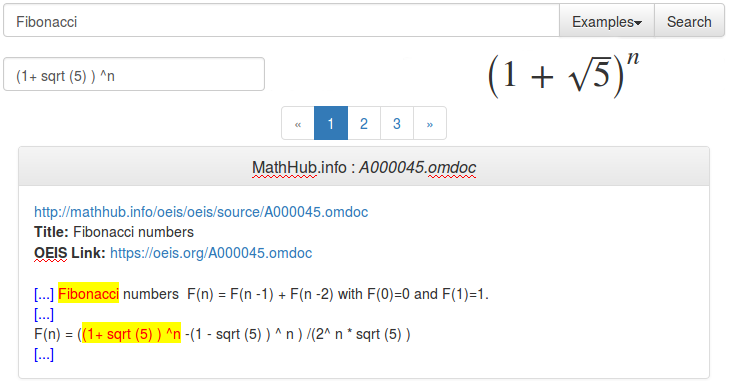
\includegraphics[scale=0.45]{search.png}
 \caption{Text and Formula Search for \oeis}\label{fig:search}
\end{figure}

To produce the harvest of the \oeis library for \mwss we export the \html from the content imported
into \mmt. We reuse the \mmt presentation framework and only enhance it with \oeis-specific technicalities such as
sequence name or \oeis link. For the formula converter we use the same parser used for \oeis formulas and described
above, except extended with one
grammar rule for \mwss \emph{query variables}. We then forward the resulting formula in \mmt to produce the
presentation
(\mathml) and return it to the \mwss frontend.  The web-server infrastructure, needed to communicate with \mwss, is
provided
by \mmt and we just extend it. Figure \ref{fig:search} shows (a part of) the current interface answering a query about
Fibonacci numbers. The search system is available at \url{http://ash.eecs.jacobs-university.de:9999/}.



%%% Local Variables:
%%% mode: latex
%%% TeX-master: "report"
%%% End:

\section{Search} \label{sec:Search}
%\subsection{Realizing Text and Formula search for \oeis}

{\mws} (\mwss) \cite{KohPro:man13} is an open-source, open-format, content-oriented search
engine for mathematical expressions. We refer to \cite{KohPro:man13} for details.

To realize the search instance in \mwss we need to provide two things:
\begin{compactenum}
 \item A \emph{harvest} of \mathml-enriched \html files that the search system can resolve queries against.
 The content-\mathml from the files will be used to resolve the formula part of the query while the rest of the \html
will be used for the text part. The harvest additionally requires a configuration file
that defines the location in the \html files of \mwss-relevant metadata such as the title, author or URL of the
original
article. This, together with the \html itself is used when presenting the query results.
 \item A \emph{formula converter} that converts a text-based formula format into \mathml. This will be used so that
 we can input formulas for searching in a text format (in our case \oeis-inspired ASCII math syntax) rather than
 writing
 \mathml directly.
\end{compactenum}

\begin{figure}
\centering
 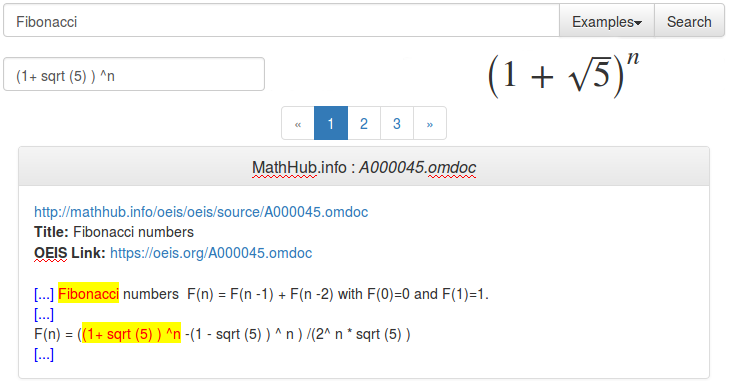
\includegraphics[width=15cm]{search.png}
 \caption{Text and Formula Search for \oeis}\label{fig:search}
\end{figure}

To produce the harvest of the \oeis library for \mwss we export the \html from the content
imported into \mmt. We reuse the \mmt presentation framework and only enhance it with
\oeis-specific technicalities such as sequence name or \oeis link. For the formula
converter we use the same parser used for \oeis formulas and described above, except
extended with one grammar rule for \mwss \emph{query variables}. We then forward the
resulting formula in \mmt to produce the presentation (\mathml) and return it to the \mwss
frontend.  The web-server infrastructure, needed to communicate with \mwss, is provided by
\mmt and we just extend it. Figure \ref{fig:search} shows (a part of) the current
interface answering a query about Fibonacci numbers. The search system is available at
\url{http://oeissearch.mathweb.org}.



%%% Local Variables:
%%% mode: latex
%%% TeX-master: "../report"
%%% End:

  \section{Enriching the \oeis with a Theory Graph} \label{sec:Enrich}

In the proceeding subsections we first propose a way of representing the \oeis Theory Graph. Then, we discuss an
approach of finding views and discuss the results we get from it.

\subsection{Representing \oeis in Theory Graph} \label{sec:Representation}

First, we need to define the \emph{theory} in the context of \oeis, hence we need to define all the notions related
to the \emph{theory} in this context. We propose the following way to define the theory of a sequence.\\
A sequence $S$ has a corresponding theory which has a typed symbol, $S : nat \mapsto int$ to represent the function
symbol and all the functions are expressed as axioms. Assuming the sequence $S$ contains two functions $f(n)$ and $g
(n)$ the axioms would be:
\begin{equation}
\begin{split}
S_{f}: S &= \lambda n. \ f(n) \\
S_{g}: S &= \lambda n. \ g(n)
\end{split}
\end{equation}

%Where $[n]\ g\ n$ is the equivalent of $\lambda n.gn$.

Now that we have a way to define the theory, we will show  the other notions related to it. The theory inclusions are
 practically the same as in other contexts. The theory $T_i$ that includes theory $T_j$ imports all the symbols of
 theory $T_j$ and they become available in theory $T_i$. An implication of this theory representation is that we can
 represent relations between sequences as views between their corresponding theories.\\
Assume that we have two sequences $S_i$ and $S_j$ and that their respective theories are $T_i$ and $T_j$. If their
corresponding functions are $f$ and $g$, respectively, then theory $T_i$ and $T_j$ can be represented as:\\

\[ T_i = \begin{cases} S_i : nat \mapsto int \\ S_{f} : S_i = f   \\
\end{cases} \]  and
\[ T_j = \begin{cases} S_j : nat \mapsto int \\ S_{g} : S_j = g   \\
\end{cases} \]


If $f$ and $g$ are related through a function $h : (nat \mapsto int) \mapsto (nat \mapsto int)$ such that, $f = h(g)$
 then one can construct a view $\phi$ from $T_i$ to $T_j$, and that is:

\begin{equation}
\phi = \begin{bmatrix} S_i \mapsto h\ S_j  \\ S_{f} \mapsto  \text{proof that the axiom holds in } T_j \end{bmatrix}
\end{equation}

One can easily construct the proof given that we know the function $h$.

A more general case is when the relation occurs between two functions of different sequences but one of the sequences
 has more than one representing function.
Let $S_i$ be a sequence which has $m$ functions and the corresponding theory $T_i$. Since all the functions represent
 the same sequence then they must be equal. We take these as theorems stating the equality of the $m$ functions with
 each other. These are then contained in a special theory $U$, included by all the corresponding theories of sequences. \\
To show this general case, let us have the sequence $S_i$ as above, and a sequence $S_j$ with $k$ functions. Let
there be a relation $h: (nat \mapsto int) \mapsto (nat \mapsto int)$ that maps one of the functions of $S_j$, say
$g_1$ to function $f$ from $S_i$. A view $\theta$, from $T_i$ to $T_j$ needs to have proofs for all the axioms of
$T_i$ under the symbol assignments in $\theta$. The symbol assignment is the same as in the case when $S_j$ had only
one function. From the available theorems in theory $U$ we get $g_1=g_2=...=g_k$. Thus, from $f=h(g_1)$ we get $f=h
(g_i)$ for $i$ in $\{1,\ldots, k\}$, which simplifies the matter to the already explained initial case.
We can encode similarly the case when the view is based on the generating functions.

\subsection{Algorithm}

The current representation of the library allows us to access the formulas present in the \oeis documents. Although
the representing functions are available, we do relation searching on the level of the ordinary generating functions.
 The approach we follow is mathematically simple. We will show three methods, each building on top of the previous one.

\paragraph{Method 1} In this case, we \emph{normalize} the ordinary generating functions of the sequences and check
for equality between the normalized expressions.
The normalization rules are defined as follows:

    \begin{prooftree}
    \AxiomC{$cG$ \ \ \ $c$ - constant \ \ \ $G$ - generating function}
    \RightLabel{\rulename{Const}}
    \UnaryInfC{$G$}
    \end{prooftree}

    \begin{prooftree}
    \AxiomC{$x^nG$ \ \ \ $x$ - the indeterminate of $G$ \ \ \ $G$ - generating function}
    \RightLabel{$\rulename{Unshift}_n$}
    \UnaryInfC{$G$}
    \end{prooftree}

    \begin{prooftree}
    \AxiomC{$P/Q$ \ \ \ $P,Q$ - polynomials}
    \RightLabel{\rulename{Sort}}
    \UnaryInfC{($\sum_{i=0}^{n} p_ix^i) / (\sum_{i=1}^{m} q_ix^i)$ \ \ \ $p_n > 0$ \ \ \ $q_n > 0$}
    \end{prooftree}

The rules are composed in the same order as defined above to form the method \emph{normalize}.
The first two rules are self-evident in what they are supposed to achieve. Rule \rulename{Sort} is used for sorting
the polynomials based on ascending powers of $x$. We add an extra condition on the sign of the highest degree term to
 normalize the sign of the polynomial.

The normalization rules entail easily interpretable relations with the pre-normalized formula. Rule \rulename{Const}
is removing the multiplying constant. Multiplying an ordinary generating function by a constant is equivalent to
multiplying each term of the sequence by that number.
Since multiplying by $x^n$ is the same as shifting the sequence the \rulename{Unshift}$_n$ is normalizing the shift.

Let $B$ (before) be the pre-normalized ordinary generating function, and $A$ (after) the normalized one. Also, let
$\hat{B}(n), \hat{A}(n)$ be the representing functions of the sequence represented by $B,A$, respectively. Then, the
relations that the normalizing rules entail are:

\begin{enumerate}
\item Rule \rulename{Const}: $\hat{A}(n) = \frac{1}{c}\hat{B}(n)$.
\item Rule \rulename{Unshift}$_k$: $\hat{A}(n) = \hat{B}(n+k)$ given that $x^k$ was removed.
\item Rule \rulename{Sort}: $\hat{A}(n) = \hat{B}(n)$.
\end{enumerate}

Intuitively, in this case we are checking if sequences are scaled and/or shifted versions of each other. These
relations are not meant to be interesting or new.

\paragraph{Method 2} In this case we check if a sequence can be expressed as a sum of other sequences existing in the
 \oeis, possibly \emph{normalized} and \emph{transformed}.

A simplified algorithm roughly follows this pseudocode:
\newpage
\begin{lstlisting}[style=myScalastyle]
foreach sequence
    foreach ogf in ordinaryGeneratingFunction(sequence)
        hashSet.put(normalize(ogf))

foreach sequence
    foreach ogf in ordinaryGeneratingFunction(sequence)
        pdf = partialFractionDecomposition(ogf)
        partialFractions = decompose(partialFractions(pfd))
        relationsExists =
            forall pgf in partialFractions
                transformedPartialFractions = normalize(applyTransformations(pgf))
                transformedPartialFractions.intersection(hashSet).nonEmpty
        if (relationsExists)
            print relations
\end{lstlisting}

We will now explain the functions that we are using above.


\begin{wrapfigure}{r}{0pt}
\begin{tikzpicture}[framed]
\node[draw, circle]      (Ti)        {$A_1$};
\node[draw, circle]      (Tj)       [right=of Ti] {$A_2$};
%Lines
\draw[dashed, latex-] (Tj.west) -- (Ti.east);
\end{tikzpicture}
\caption{Relations of \emph{Method 2}}\label{fig:directRelations}
\end{wrapfigure}

Let $GF_n$ be one of the ordinary generating functions of sequence $A_n$. The partial fraction decomposition
(\emph{partialFractionDecomposition}) applied on an ordinary generating function would leave us with:

\begin{equation}
 GF_n = \sum_{j=1}^{n} G_j \label{eq:pfd}
\end{equation}
where $G_j$ is also an ordinary generating function. The function \emph{partialFractions} then takes that sum and
extracts the summands, in this case, the partial fractions (ordinary generating functions) $G_j$. The function
\emph{decompose} does a further step of decomposition. If $G_j = \frac{P}{Q}$ where $P,Q$ are polynomials ( $P =
\sum_{i=0}^{n} a_ix^i$) then it rewrites $G_j = \sum_{i=0}^{n} \frac{a_ix^i}{Q}$. These summands are then considered
'partial fractions', too.

\begin{wrapfigure}{r}{2.8cm}
\begin{tikzpicture}[framed]
\node[draw, circle]      (T)                              {$N$};
\node[draw, circle]        (Tj)       [right=of T] {$A_1$};
\node[draw, circle]      (Ti)       [below=of T] {$A_2$};

%Lines
\draw[latex-] (Ti.north) -- (T.south);
\draw[latex-] (Tj.west) -- (T.east);
\draw[dashed, latex-] (Tj.south) -- (Ti.east);
\end{tikzpicture}
\caption{Relations of \emph{Method 3}}\label{fig:transitiveRelations}
\end{wrapfigure}


The transformations are \emph{integration, differentiation} and \emph{unit}.
The transformations are selected such that expressions that match under these transformations can be easily related
both mathematically and semantically.

Similarly, let $B$ be the pre-transformed ordinary generating function, and $A$ the transformed one. Let $\hat{B}(n),
 \hat{A}(n)$ be the representing function of the sequence represented by $B,A$, respectively. Then, the relations
 that the transformation rules entail are:

\begin{enumerate}
\item Integration: $\hat{A}(n) = \frac{1}{n}\hat{B}(n-1)$.
\item Differentiation: $\hat{A}(n) = n\hat{B}(n+1)$.
\item Unit: $\hat{A}(n) = \hat{B}(n)$.
\end{enumerate}

If $GF_n$ is the ordinary generating function of sequence $A_n$, $c_i$ a real constant, $p \in \{-1,0,1\}$ and $k_i$
an integer, the algorithm would try to find relations of the form:
\begin{equation}
A_j(n) = \sum_{i=0}^{n} c_i n^p A_i(n-k_i)
\end{equation}

In this case we will be finding what we call \emph{direct relations}. So there is a direct \emph{view} between the
sequences (Fig. \ref{fig:directRelations}).


\paragraph{Method 3}

In this case we do not restrict the generating functions to be representing existing \oeis sequences. Instead, we
search if two ordinary generating functions have a common partial fraction in their summation of partial fractions
(Fig. \ref{fig:transitiveRelations}).


% \newpage
The simplified algorithm is given by the pseudocode below.
\begin{lstlisting}[style=myScalastyle]
foreach sequence
    foreach ogf in ordinaryGeneratingFunction(sequence)
        pfd = partialFractionDecomposition(ogf)
        partialFractions = decompose(partialFractions(pfd))
        foreach pgf in partialFraction
            transformations = normalize(applyTransformations(pgf))
            foreach transformed in transformations
                if transformed exists in hashSet
                    print relation
                else
                    add pgf to hashSet
\end{lstlisting}

As an example, let us take two sequences $A_1$ and $A_2$ and their corresponding ordinary generating functions $GF_1$
 and $GF_2$. Let $N$ be a partial fraction and $M,S$ sums of partial fractions. Moreover, for any $G$, if $G$ is an
 ordinary generating function, let $\hat{G}$ denote the representing function of the same sequence that $G$ represents. If
\begin{align}
GF_1 &= M + \int N \\
GF_2 &= S + N
\end{align}
then from the relations defined above and assuming that the representing functions exist, we can carry over the
relation to the representing functions:
\begin{align}
\hat{GF_1}(n) &= \hat{M}(n) + \frac{1}{n}\hat{N}(n-1) \\
\hat{GF_2}(n) &= \hat{S}(n) + \hat{N}(n)
\end{align}
Which then can be solved to give:
\begin{align}
\hat{GF_2}(n) = \hat{S}(n) + (n+1)(\hat{GF_1}(n+1) - \hat{M}(n+1)) \label{eq:transform}
\end{align}

Notice that the step of carrying over the relation between generating functions, to the corresponding representing
functions assumes that the representing functions exist, which is not always the case. Nonetheless, it is worth
noticing that the last equation is independent of $\hat{N}$.

\subsection{Implementation and Evaluation}

\begin{figure}[!h]
\begin{subfigure}{0.3\textwidth}
\centerline{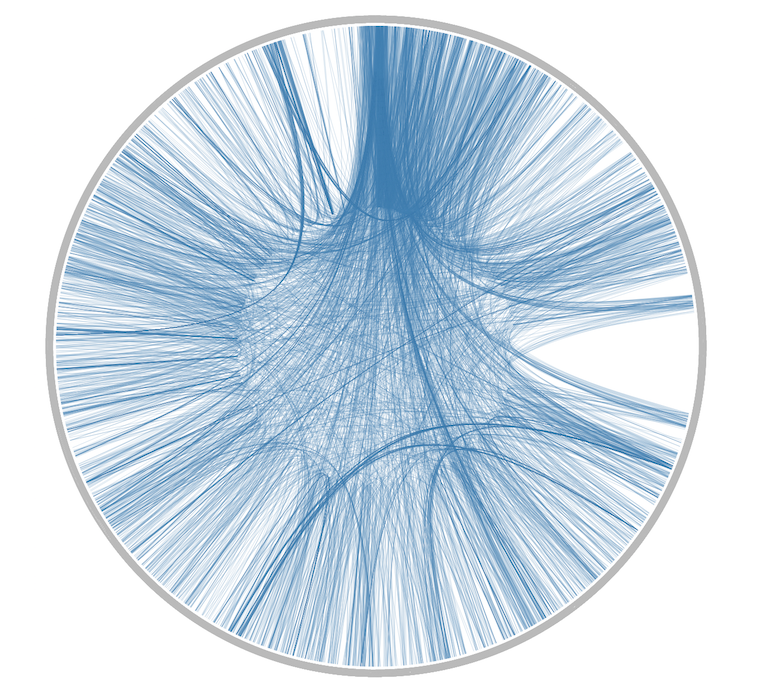
\includegraphics[scale=0.2]{before}}
\caption{OEIS Theory Graph of Explicit Views \label{fig:before}}
\end{subfigure}
\begin{subfigure}{0.3\textwidth}
\centerline{
\includegraphics[scale=0.22]{after}}
\caption{OEIS Theory Graph of Inferred Views using Method 3 \label{fig:after}}
\end{subfigure}
\begin{subfigure}{0.3\textwidth}
\centerline{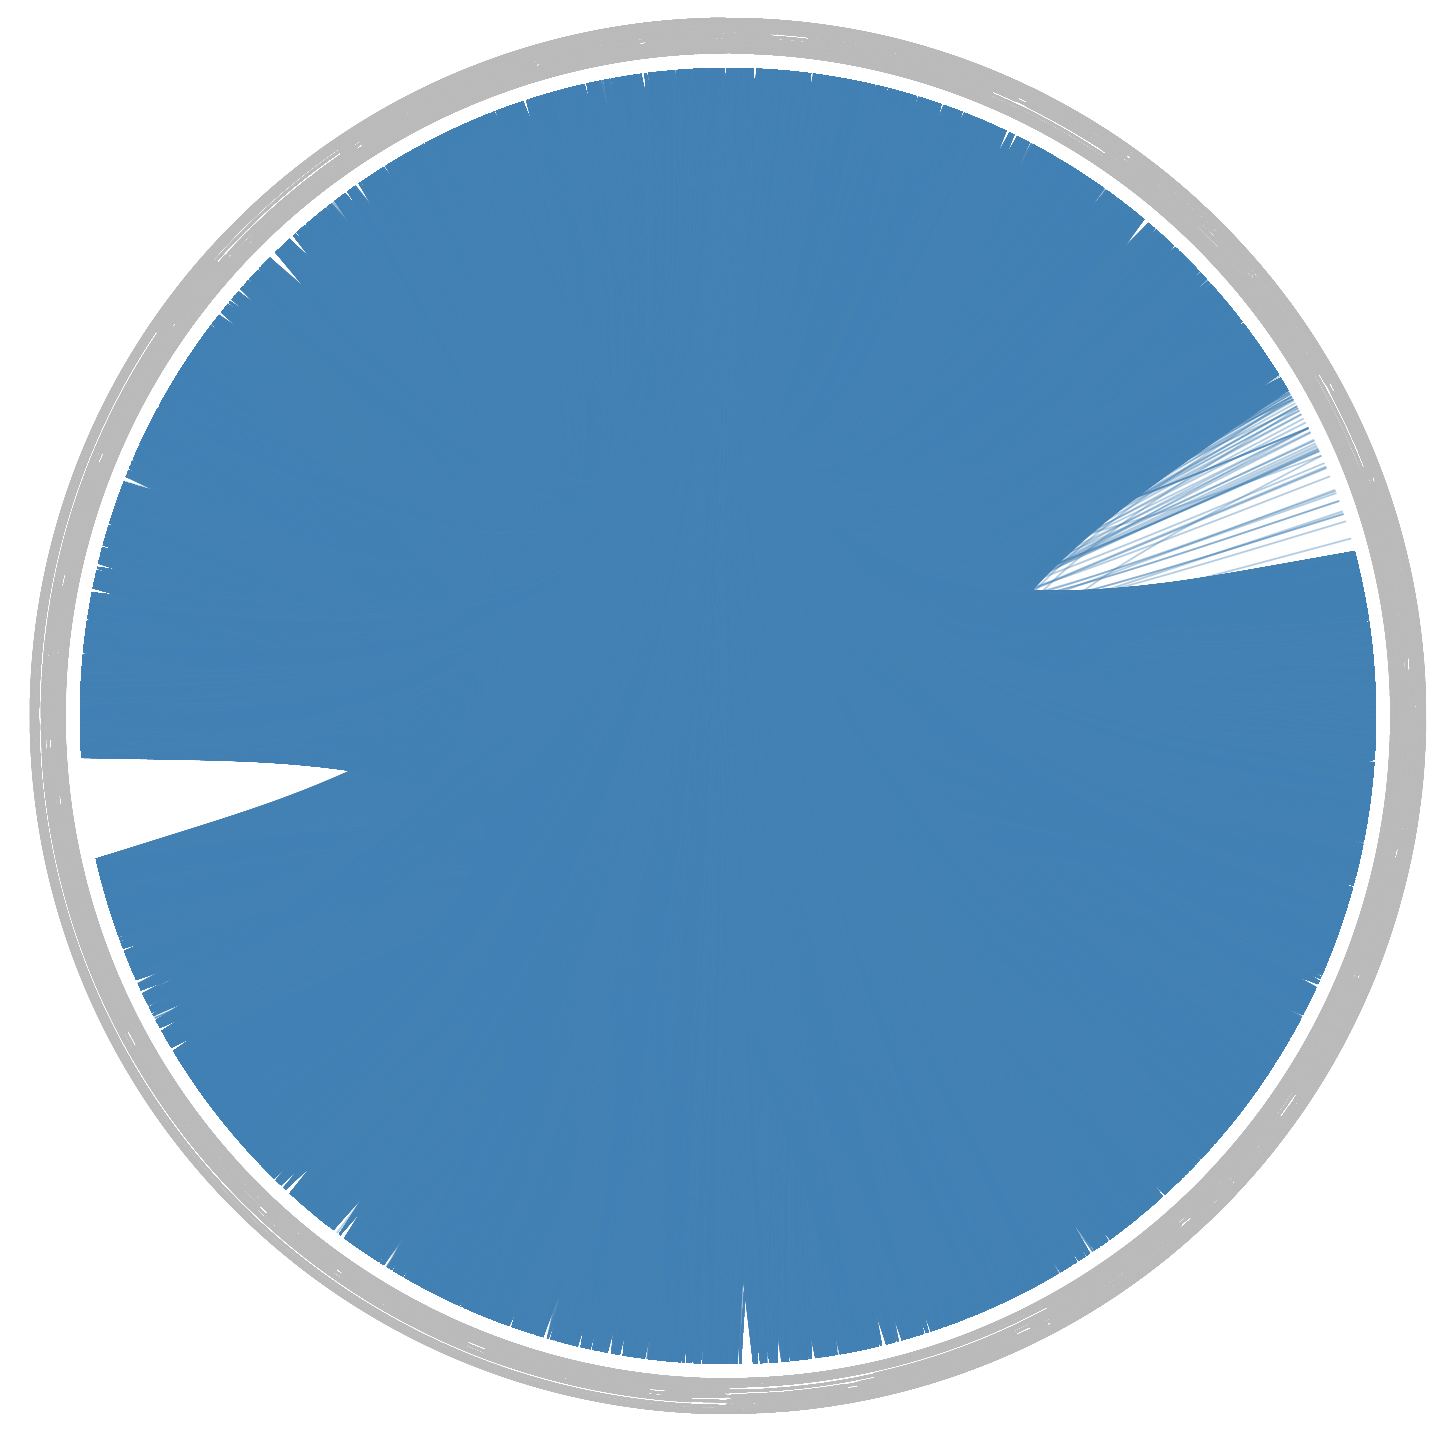
\includegraphics[scale=0.17]{after2}}
\caption{OEIS Theory Graph of Inferred Views using Method 2 \label{fig:after2}}
\end{subfigure}
\medskip
\small

The points around the circle represent the theories and the blue lines views between them. The theories presented
here are only the ones for which we have parsed the generating functions.

\caption{OEIS Theory Graphs}

\end{figure}

The relation finder is implemented in Scala and is available at \url{https://github.com/eluzhnica/ISFA}. The page
will be kept up to date with results. The implementation of the \emph{normalization} rules makes use of the parsing
tree of the expression that we get from the parsing phase. The \emph{transformations} are done using SageMath as a
math engine. Our Scala code communicates with a local SageMath server using a REST API. The SageMath calls are cached
 in Mongo for practicality during development.

Below, we walk through some examples of the relations found from each method.
\paragraph{Method 1}
This is more of a sanity check of the algorithm. Due to the nature of these relations, these are self-evident
relations. Additionally, these relations can be effectively searched utilizing a numerical method. An instance that
our algorithm finds is that sequence $A001478(n) = -A000012(n)$. Sequence $A001478$ is the sequence of the negative
integers, while $A000012$ is the sequence of positive integers.

\paragraph{Method 2}
An example of this method, which we have submitted and it is accepted in the \oeis (\url{https://oeis.org/A037532}),
is as follows.
Sequence $A037532$ has an ordinary generating function:
\begin{align}
\frac{x(1+x+2x^2)}{(x-1)(7x-1)(1+x+x^2)} \stackrel{\text{PFD}}{=} &\frac{1}{57}\frac{5x + 3}{x^2 + x + 1} -
\frac{\frac{29}{171}}{7x- 1} + \frac{\frac{2}{9}}{x - 1} \\
\stackrel{\text{Decomp.} + \rulename{Sort}}{=} &\frac{1}{57}\frac{5x}{1+x+x^2} + \frac{1}{57}\frac{3}{1+x+x^2} -
\frac{\frac{29}{171}}{-1 + 7x} + \frac{\frac{2}{9}}{-1 + x}
\end{align}
Sequence $A049347$:
\begin{equation}
\frac{1}{1+x+x^2}
\end{equation}
Sequence $A000420$:
\begin{equation}
\frac{1}{1-7x} \stackrel{\rulename{Sort}}{=} -\frac{1}{-1+7x}
\end{equation}
Sequence $A000012$:
\begin{equation}
\frac{1}{1-x} \stackrel{\rulename{Sort}}{=} -\frac{1}{-1+x}
\end{equation}

It is clear that the relation that can be derived here is:
\begin{equation} \label{eq:accepted}
A037532(n) = \frac{5}{57}A049347(n-1) + \frac{3}{57}A049347(n) + \frac{29}{171}A000420(n) - \frac{2}{9}
\end{equation}
There is one subtlety that needs to be explained. The sequence with ordinary generating function $\frac{1}{1-x}$ is
the sequence $(1,1,1, \ldots)$. However, for simplicity we write down $\frac{2}{9}$ instead of $\frac{2}{9}A000012(n)
$. However, our algorithm does not do that.

\paragraph{Method 3} An example relation is shown below.

Sequence $A257890$ has a generating function:
\begin{equation}
\frac{(x^2-x+1)(x^2-3x+3)}{(x-1)^6} = \frac{1}{(x - 1)^2} + \frac{1}{(x - 1)^4} + \frac{1}{(x - 1)^6}
\end{equation}
Sequence $A257199$ has a generating function:
\begin{align}
\frac{x(1 - x + x^2)}{(1 - x)^6} = \frac{1}{(x - 1)^3} + \frac{2}{(x - 1)^4} + \frac{2}{(x - 1)^5} + \frac{1}{(x - 1)
^6}
\end{align}

Clearly, $\frac{1}{(x-1)^6}$ is in common. But also, $-5\int \frac{1}{(x-1)^6} dx = \frac{1}{(x-1)^5}$, which makes
it possible to express a relation through $\frac{1}{(x-1)^5}$, too. In this case we can use the technique used in
Equation \ref{eq:transform} to carry over the relation to the representing functions since the representing functions
 of the corresponding sequences are known. Hence, we get the following relation:
\begin{multline}
A257890(n) = A000027(n+1) + A000292(n+1) \\
- \frac{n+1}{10}(A257199(n+1)
 + A000217(n+2) - 2*A000292(n+2) - A000389(n+6))
\end{multline}
Nonetheless, in the general case the relation cannot be always carried over to the representing function, so the
relation would only be in the level of the generating function.

Since our parser runs over all the formulas of \oeis, we have extracted the existing explicit relations in \oeis and
made a graph (Figure \ref{fig:before}) showing the existing connections between sequences .
The second method enriches the theory graph as shown in Figure \ref{fig:after2} and the third method as shown in
Figure \ref{fig:after}).

\begin{center}
 \begin{tabular}{||c | c||}
 \hline
 Parsed Generating Functions & 39\ 218 \\
 \hline
 SageMath syntax-proof Generating Functions & 22\ 757 \\
 \hline
 Verified Ordinary Generating Functions & 21\ 872 \\
 \hline
 Parsed Ordinary Generating Functions &  35\ 953 \\
 \hline
 SageMath verified Ordinary Generating Functions & 13\ 400 \\
 \hline
 Method 1 relations & 4\ 859 \\
 \hline
 Sequences in Method 1 relations & 853 \\
 \hline
 Method 2 relations & 262\ 751\ 850\\
 \hline
 Method 3 relations & 98\ 401 \\
 \hline
\end{tabular}
\end{center}

The number of parsed generating functions is self-explanatory. The generating functions are extracted from the formulae that were parsed during the parsing phase.
These generating functions are of all kinds - ordinary, Dirichlet, exponential generating functions 
just to name a few. However, we were only interested in the ordinary generating functions. 
Since the parser is not guaranteed to produce correct results, nor the filtering of the ordinary
generating functions, two verification methods are employed. The first verification method is used to filter the generating functions that we can compute on. The second verification method is used to 
filter the ordinary generating functions that are actually correct and that we can rely to generate
new relations. These are the generating functions that the relation-generation algorithms use. 
First, we translated the parsed generating functions in SageMath syntax and checked if they were accepted from SageMath. We name the generating functions that pass this test as 'SageMath syntax-proof Generating Functions' in the table above. From a manual inspection we notice that most of the generating functions that do not pass this test are due to external references to unknown functions. For instance, $1+Q(0)$ where the function $Q(n)$ is defined later on in the sequence document. Currently, we do not resolve these references.
Second, the parsed ordinary generating functions are used to generate the first 8 terms of the sequence and then matched against the first terms (fetched from \oeis). This is important to set a basis for correct relations. In fact, this is also
important to further verify the parsing accuracy aswell as the \oeis data. 
From an inspection of $70$ ordinary generating functions that failed the verification phase (data available at: \url{https://github.com/eluzhnica/oeis_gf/blob/master/failed}), only 1 was found to have been wrongly parsed. It was due to an unexpected mix of words and formulae.
On the other hand, from another (incomplete) inspection of the same data we noticed 18 incorrect generating functions in the \oeis.  Two of them were already fixed, we just had an older copy of the \oeis. The rest were mostly the generating function not matching the shift/initial terms. However, there was also a case where the generating function matched only the first 5 terms but not the rest. 
Finally, we also made a SageMath module where users can access the ordinary generating functions of the sequences and made it accessible at \url{https://github.com/eluzhnica/oeis_gf}.
% Most of the generating functions that are not qualified are due to  that were not being accepted were because they referred to some other functions. For
%   instance, $1+Q(0)$ where the function $Q(n)$ is defined later on in the sequence document. We currently do not
%   resolve these references.

Method 1 reports $4859$ relations of that kind. However, in total only $853$ sequences are involved in these relations.

One can notice that there is a plethora relations generated from the second method. However, this is expected.
Take for instance, $G = A + B + C + D$, where $G$ is the generating function of a sequence, and $A,B,C, D$ are the
partial fractions. If each partial fraction represents an \oeis sequence under every transformation (unit, derivate,
integrate), then the number of relations that we can form is actually $3^4$. Clearly,
the number of relations per generating function are bound by the exponential function $f(n) = 3^n$ where $n$ is the 
number of partial fractions (including the partial fractions that come from \emph{decomopose}). Since there are generating functions
with up to $22$ partial fractions, the big number of relations is not a big surprise.

Out of three relation submissions to the \oeis, two relations are already accepted
\cite{oeis-accepted-1,oeis-accepted-2} under the author's name. One of them has already
been presented in Equation \ref{eq:accepted} and the other relation is
$A001787(n) = A007283(n) \frac{n}{6}$ which can be found at
\url{https://oeis.org/A001787}. The unaccepted submission was not perceived to add new
information since a similar relation was already present. The submitted relations were
selected randomly.

%%% Local Variables:
%%% mode: latex
%%% TeX-master: "../report"
%%% End:

\section{Improving the OEIS Formula Language} \label{sec:Improve}

Section \ref{sec:form-parser} introduced the problems when parsing the \oeis. In this section we are going to show an
 improved formula language and the parser for it.

OEIS has a strong policy advocating human readable math syntax. Users have a pretty strong autonomy on what notation
they use.
In the FAQ of OEIS we can see these:

\begin{lstlisting}
Q: Is it OK to use LaTex or Maple notation in equations?
A: No, please don't!

Use notation that can be understood by humans.
Say     (1+x)/(1-x)     not     $\frac{(1+x)}{(1-x)}$.
Say     n^2/2     not     1/2n^2.
Say     A/(B*C*D)     not     A/B/C/D
Say     sigma     not     $\sigma$.
\end{lstlisting}

The above explicitly suggests a human readable format and implicitly not using any sort of delineation. Furthermore,
the FAQ also contains:

\begin{lstlisting}
Q: How should I indicate summations?
A: There are many acceptable ways to do this.

All of the following examples are OK.

sum_{i=1..n} i^2 + i

sum_i=1..n (i^2+i)

sum_{d|n} d^3

sum_{ 2 <= p <= n, p prime} p^2

Other styles also acceptable, as long as they are clear!
\end{lstlisting}
This offers too much autonomy in the choice of constructs and even the proposed notations lead to ambiguous usages.
For instance, in the expression below, it is unclear if the first expression equivalent to any of the ones below it.

\begin{lstlisting}
x^2 + sum_{i=1..n} i^2 + 2
x^2 + sum_{i=1..n} (i^2) + 2
x^2 + sum_{i=1..n} (i^2 + 2)
\end{lstlisting}


While human readability is certainly important, there better ways to achieve it while making it easier for the
parsers to mine the invaluable resources in the \oeis. In fact, once the parsers successfully parse the formulas, we
can then have MathML presentations of the formulas. In this section we show the an improved language for which we
have implemented a parser. The approach should be read having in mind the practicality of adopting the implementation
 from the \oeis which explains the choice of a less rigorous language. We only address a part of the language,
 specifically the part that is attempted by the current parser.

\subsection{Language}
We categorize two levels of ambiguity:

\begin{enumerate}
    \item Having no clearly defined semantic interpretation. For instance, in $phi(x+2)$, the  function that $phi$
    refers to is not defined.

    \item Having two or more clearly defined and distinct semantic interpretations of an expression. An example is
    $pi(x+2)$, where $pi$ could be function or a variable.
\end{enumerate}

The level of severity in terms of ambiguity is debatable. If the goal is computing with these expressions, then the
second ambiguity might be more severe than the first. In the example above, if we know the function to which $pi$
refers to, then it is possible to compute all possible semantic interpretations of the expression.

In the \oeis context, the first level is a bigger issue, mainly due to the fact that there are special sections in
\oeis for computational purposes. These sections contain executable code for Mathematica, Maple etc.

\oeis has to two different formats, the \emph{internal} format and the \emph{text} format which is shown to the users
. Our modifications are applicable to the internal format, while the text format does not necessarily change.

\paragraph{Delineating formulas} Currently, the majority of failures of the existing parser are attributed to lack of
 delineation.
So we add deliniators to the internal format. Once the formulae are parsed, the text format can optionally change to
show them in MathML.

\paragraph{Ambiguity and Open Set of Primitives} The new language disallows implicit multiplication. However, the
explicit multiplication will only show up in the internal format, while the text format still includes the implicit
multiplication.

\begin{wrapfigure}{r}{8.0cm}
\vspace{-0.5cm}
\begin{center}
\begin{tabular}{|lll|}
\hline
$\mathit{S}$ & \bbc & $\mathit{Func}\; | \mathit{Rel}\; | \mathit{Const}\; | \mathit{Esc}$\\
$\mathit{Func}$ & \bbc & $\textit{:func}\; \mathit{Name}\; \mathit{Arg} \; \mathit{Form} \; \mathit{Prec} \;
\mathit{Desc} $ \\
$\mathit{Rel}$ & \bbc & \textit{:rel}$\; \mathit{Name}\; \mathit{Form} \; \mathit{Prec} \; \mathit{Desc} $ \\
$\mathit{Const}$ & \bbc & \textit{:const}$\; \mathit{Name}\; \mathit{Desc} $ \\
$\mathit{Esc}$ & \bbc & $\textit{:esc}\; \mathit{Name}\; \mathit{Desc} $ \\
$\mathit{Name}$ & \bbc & Name of the function \\
$\mathit{Arg}$ & \bbc & $\mathtt{(\mathit{W}, ..., \mathit{W})|(\mathit{W}, ..., \mathit{W}) \mathit{Arg}} $ \\
$\mathit{Form}$ & \bbc & \textit{prefix | suffix | infix} \\
$\mathit{Prec}$ & \bbc & [$1$-$2^{31}$] \\
$\mathit{Desc}$ & \bbc & Description \\
$\mathit{W}$     & \bbc & [a-zA-Z0-9\_] \\
\hline

\end{tabular}
\caption{Grammar of \oeis language theory}\label{fig:theory-form}
\end{center}
\end{wrapfigure}

The other problems are solved by having an explicit source of knowledge. This means having a document which lists the
 in fix, postfix, relational operators and the constants. This is what we call the \emph{language theory} of an \oeis
 document. These theories do not have complex inheritance system. They can be either global in scope to the whole
 \oeis, or local, only in the scope of one \oeis document. This is reduces the reusability, however with this we
 intend to increase the readability and user friendliness since there are usually a very limited number of operators
 defined per document. These definitions follow a simple format, declaring the operator, the argument pattern, the
 type, the precedence and the meaning in a few words.
Assuming the description is good the definitions can be manually converted into more formal notations to be used for
computation purposes.
Other forms of ambiguity are generally solved in the same way: we get closer to the rigorous math notation. For
instance, the power operators need to be properly bracketed - \verb|T^y(x^2+2)| should be written as \verb|(T(x^2+2))^y|.
 Nonetheless, unbracketed function application is allowed since it is already disambiguated by disallowing
implicit multiplication.

Due to the natural language usage we have unusual expressions. For instance we can spot expressions of the form:
\begin{verbatim}
    x^y + 2*triangular number
    2*x + perfect square
    sum_{i in fibbonaci numbers}
\end{verbatim}
We have the constructs that we call \emph{escapers} to allow creating these expressions. With escapers the syntax
would then become:

\begin{verbatim}
    x^y + 2*{{triangular number}}
    2*x + {{perfect square}}}
    sum_{i in {{fibbonaci numbers}}}
\end{verbatim}

These constructs can contain natural language, however they still have to be defined in the theory of the document.

Below is an example definition of the theory for the sequence \verb|A000045| which is partially shown in Section ??.

\renewcommand{\lstlistingname}{Theory}

\begin{lstlisting}[label=lst:theoryA000045,caption=Example theory for A000045]
:func     sqrt    (x1)        prefix  1   The square root of x1
:func     sum     (x1, x2)    prefix  1   Sum over x1 for values defined in x2.
:const    pi                              The number 3.14159
:rel      >=                  infix   2   Greater than or equal
:func     +                   infix   1   Sum
:rel      to                  infix   2   Range
:func     F                   prefix  1   The Fibonacci function
\end{lstlisting}

We have shown all of the definitions in one theory for simplicity. In a normal setting, some of them would be defined
 in the global theory. We have also omitted some operators for brevity.
Using the rules above the formula language for the sequence document would then be transformed as shown below.

\begin{lstlisting}[caption=Adjusted A000045 based on Theory \ref{lst:theoryA000045}]
%F A000045 $F(n) = ((1+sqrt(5))^n-(1-sqrt(5))^n)/(2^n*sqrt(5))$
%F A000045 G.f.: $Sum_{n>=0}{x^n * Product_{k,1 to n} {(k + x)/(1 + k*x)}}$. - _Paul D. Hanna_, Oct 26 2013
%F A000045 This is a divisibility sequence; that is, if n divides m, then a(n) divides a(m)
\end{lstlisting}

Notice that the last line could very easily be delineated as math, but we did not do it
for illustration purposes.

A complete definition for the theory definition language has been given in Figure
\ref{fig:theory-form}. The defined operators are considered to be left associative.

\paragraph{Implementation} The parser of the new language and the parser of the theory
definition language have been implemented using the Packrat Parser \cite{packrat} in
Scala. The theory definitions are first parsed and then fed to the parser for the formula
language.  The current limitation of the formula language parser is that it doesn't
support the operator precedences. It parses the prefix, infix and postfix operators in
order.


%%% Local Variables:
%%% mode: latex
%%% TeX-master: "report"
%%% End:

\section{Conclusion}\label{sec:concl}

We have shown how to extend the Math-in-the-Middle framework for integrating systems to mathematical data bases like the \lmfdb. 
The main idea is to embed knowledge sources as virtual theories, i.e. theories that are not -- theoretically or in practice -- limited in the number of declarations and allow dynamic loading and processing. 
For accessing real-world knowledge sources, we have developed the notion of codecs and integrated them into the MitM ontology framework. 
These codec's (and their MitM types) lift knowledge source access to the MitM level and thus enable object-level interoperability and allow humans (mathematicians) access using the concepts they are familiar with. 
Finally, we have shown a prototypical query translation facility that allows to delegate some of the processing to the underlying knowledge source and thus avoid thrashing of virtual theories. 

\paragraph{Related Work} Most other integration schemes employ a \textbf{homogenous approach}, where there is a master sytsem and all data is converted into that system. 
A paradigmatic example of this is the Wolfram Language and the Wolfram Alpha search engine~\cite{WolframAlpha:on}, which are based on the Mathematica kernel. 
This is very flexible for anyone owning a Matheamtica license and experienced in the Mathematica language and environment.

The MitM-based approach to interoperability of data sources and systems proposed in this paper is inherently a \textbf{heterogeneous approach}: systems and data sources are kept ``as is'', but their APIs are documented in a machine-actionable way that can be utilized for remote procedure calls, content format mediation, and service discovery. 
As a consequence, interaction between systems is very flexible.
For the data source integration via virtual theories presented in this paper this is important. 
For instance, we can just make an extension of \mmt or Sage which just act as a programmatic interface for e.g. \lmfdb. 

\paragraph{Future Work}
We have discussed the MitM+virtual theories methodology on the elliptic curves sub-base of the \lmfdb, which we have fully integrated. 
We are currently working on additional \lmfdb sub-bases. 
The main problem to be solved is to elicit the information for the respective schema theories from the \lmfdb community. 
Once that is accomplished, specifying them in the format discussed in this paper and writing the respective codecs is straightforward. 

Moreover, we are working on integrating the the Online Encyclopedia of Integer Sequences (OEIS~\cite{Sloane:OEIS,oeis}). 
Here we have a different problem: the OEIS database is essentially a flat ASCII file with different slots (for initial segments of the sequences, references, comments, and formulae); all minimally marked up ASCII art. 
In~\cite{LuzKoh:fsarfo16} we have already (heuristically) flexiformalized OEIS contents in \ommt; the next step will be to come up with codecs based on this basis and develop schema theories for OEIS.

\subsubsection*{Acknowledgements}
The authors gratefully acknowledge the fruitful discussions with other participants of
work package WP6, in particular John Cremona on the LMFDB and Dennis M\"uller on early
versions of the \ommt-based integration. We acknowledge financial support from the
OpenDreamKit Horizon 2020 European Research Infrastructures project (\#676541).

%%% Local Variables:
%%% mode: latex
%%% TeX-master: "paper"
%%% End:

%  LocalWords:  sec:concl subsubsection ommt lmfdb itemize Sloane:OEIS,oeis LuzKoh:fsarfo16 flexiformalized MitM-based textbf utilized


\chapter{FindStat Conversion}
This part will be added later. 

\newpage\printbibliography
\cleardoublepage
\begin{appendix}
\section{Related Work} \label{App:AppendixA}
OEIS has the mail server called Superseeker which tries over 120 transformation on the \oeis sequences to match
a given sequence. This has also been used to generate relations between the current sequences by running it over the
whole \oeis corpus. The steps involved in the Superseeker for a given sequence $S$ are as follows \cite{Peter}:

\begin{enumerate}
\item Do an exact match on the current \oeis sequences.
\item Test if $S[n]$ is a polynomial in $n$.
\item Test if the difference of some order ${S_d[n]}$ are periodic.
\item Test if any row of the difference table of some depth is essentially constant.
\item Form some generating functions for the sequence for some predefined types (ie. ordinary gf, exponential gf etc.)
\item Look for a linear recurrence with polynomial coefficients for the coefficients of the above 6 types of
generating functions.
\item Apply transformations to the sequence and lookup the result in the table.
\item If the original sequence is not in the table, find the 3 closest sequences in the table using the $L1$ metric.
Only those with $L1 \leq 3$ are reported.

\end{enumerate}

An approach from Peter Liu \cite{Peter} extends the search space of finding relations. While Superseeker uses the
given sequence or its transformation sequences to query the database and the queries are exact match searches, his
approach is to use the given sequence itself to query the database and the queries are not just exact matches. They
could be the linear combination of two sequences in the table, or the affine transformation of a sequence or the
polynomial of a sequence bounded by a constant. More specifically, if $S$ is a given sequence and $D$ the sequence in
 database, the searched relations are as follows \cite{Peter}:

\begin{enumerate}
\item Is there an exact match between $S$ and $T_i \in D$?
\item Is $S$ simply some sequence in the $D$ shifted?
\item Are all member of $S$ contained in some sequence $T_i \in D$?
\item Is $S$ an affine transformation of some sequence $T_i \in D$?
\item Can $S$ be written as a polynomial of degree bounded by a constant?
\item Can $S$ be written as the linear combination of two $T_i$ and $T_j \in D$?
\item Is the $S$ close to a $T_i$?
\item Does $S$ leave a constant remainder when divided by a $T_i$?
\item Does affine transformation of $S$ give a subsequence of some $T_i \in D$?
\end{enumerate}

Of course, these queries have to be efficient enough to run over the corpus and the author realizes that through
pre-processing the database, use of hashing techniques and number theory. His approach yielded some new relations
that the Superseeker could not find, speaking of the time that Peter Liu's work has been published. From query 7, the
 author found relations of the form $T_{1923} = 2*T_{825} + T_{1428}$ or $T_{1746} = 2*T_{1205}$.

While from query 4, there were more relations found and one of those is $T_{1567} = 2*T_{1049} -1 = 2*T_{616} +1 =
4*T_{391} - 3$.
\end{appendix}

%%% Local Variables:
%%% mode: latex
%%% TeX-master: "report"
%%% End:


\nocite{IanKoh:mlkmim15}
\nocite{RabKoh:WSMSML13}
\nocite{Rabe:MAGMS13}
\nocite{oeis}
\nocite{DBLP:conf/lwa/LuzhnicaIK15}
\nocite{DBLP:conf/icms/LuzhnicaK16}

\end{document}

%%% Local Variables:
%%% mode: latex
%%% TeX-master: t
%%% End:

%  LocalWords:  maketitle newpage tableofcontents newpage newcommand xspace ednote mathdb
%  LocalWords:  standardize dktheories concl printbibliography pn textit mmt mitm emph
%  LocalWords:  WPref dksbases prioritized taskref organized delivref dkstheories
%  LocalWords:  githubissuedescription
